
%(BEGIN_QUESTION)
% Copyright 2007, Tony R. Kuphaldt, released under the Creative Commons Attribution License (v 1.0)
% This means you may do almost anything with this work of mine, so long as you give me proper credit

The ratio between base flow and pigment flow in this paint-mixing control system is not fixed.  Rather, it comes from the output of an ``analytical'' controller:

$$\includegraphics[width=15.5cm]{i01737x01.eps}$$

Explain the rationale behind this ratio control system.  Also, identify what the ``other control system'' might be that drives the base control valve.

\vskip 20pt \vbox{\hrule \hbox{\strut \vrule{} {\bf Suggestions for Socratic discussion} \vrule} \hrule}

\begin{itemize}
\item{} Identify sources of {\it dead time} in this process, and which control loop(s) will have to manage despite the presence of dead time.
\item{} Analyze the effects of the base flowmeter turbine jamming, so that it does not spin even while liquid is still flowing.
\item{} Analyze the effects of the pigment flowmeter turbine jamming, so that it does not spin even while liquid is still flowing.
\item{} Assuming the AT outputs a greater signal as the paint becomes more pigmented, determine the correct action for the AIC controller.
\end{itemize}

\underbar{file i01737}
%(END_QUESTION)





%(BEGIN_ANSWER)

The purpose of this control system is to control the coloring of the paint by analyzing its color using a special instrument, which feeds its color signal to a color controller (AIC), which then automatically adjusts the ratio between base and pigment to achieve the desired output color.

\vskip 10pt

As for the ``other control system,'' it would most likely be a flow (production) controller.

%(END_ANSWER)





%(BEGIN_NOTES)


%INDEX% Control, strategies: ratio
%INDEX% Process: paint mixing

%(END_NOTES)


